% Copyright (c) 2008-2009 solvethis
% Copyright (c) 2010-2016 Casper Ti. Vector
% Public domain.
%
% 使用前请先仔细阅读 pkuthss 和 biblatex-caspervector 的文档,
% 特别是其中的 FAQ 部分和用红色强调的部分。
% 两者可在终端/命令提示符中用
%   texdoc pkuthss
%   texdoc biblatex-caspervector
% 调出。

\documentclass[openany,UTF8]{pkuthss}
\usepackage[backend = biber, style = caspervector, utf8, sorting = ecnty]{biblatex}
\setlength{\bibitemsep}{3bp}
\renewcommand*{\bibfont}{\zihao{5}\linespread{1.27}\selectfont}

\pkuthssinfo{
	cthesisname = {本科生毕业论文}, ethesisname = {Undergraduate Thesis},
	ctitle = {全自动加样系统的设计与开发}, 
    etitle = {},
	cauthor = {宋方腾},
	eauthor = {},
	studentid = {1502024142},
	date = {2019 年 5 月},
	school = {机械工程学院},
	cmajor = {机械设计制造及其自动化}, emajor = {},
	direction = {},
	cmentor = {成云平\quad 老师}, ementor = {},
	ckeywords = {first second}, ekeywords = {First, Second}
}
\addbibresource{thesis.bib}

% 普通用户可删除此段,并相应地删除 chap/*.tex 中的
% “\pkuthssffaq % 中文测试文字。”一行。
\usepackage{color}
\def\pkuthssffaq{%
	\emph{\textcolor{red}{pkuthss 文档模版最常见问题:}}

	\texttt{\string\cite}、\texttt{\string\parencite} %
	和 \texttt{\string\supercite} 三个命令分别产生%
	未格式化的、带方括号的和上标且带方括号的引用标记:%
	\cite{test-en},\parencite{test-zh}、\supercite{test-en, test-zh}。

	若要避免章末空白页,请在调用 pkuthss 文档类时加入 \texttt{openany} 选项。

	如果编译时不出参考文献,
	请参考 \texttt{texdoc pkuthss}“问题及其解决”一章
	“其它可能存在的问题”一节中关于 biber 的说明。
}

\begin{document}
	\frontmatter
	\pagestyle{empty}
	\maketitle
	%\cleardoublepage
	% Copyright (c) 2008-2009 solvethis
% Copyright (c) 2010-2017 Casper Ti. Vector
% All rights reserved.
%
% Redistribution and use in source and binary forms, with or without
% modification, are permitted provided that the following conditions are
% met:
%
% * Redistributions of source code must retain the above copyright notice,
%   this list of conditions and the following disclaimer.
% * Redistributions in binary form must reproduce the above copyright
%   notice, this list of conditions and the following disclaimer in the
%   documentation and/or other materials provided with the distribution.
% * Neither the name of Peking University nor the names of its contributors
%   may be used to endorse or promote products derived from this software
%   without specific prior written permission.
%
% THIS SOFTWARE IS PROVIDED BY THE COPYRIGHT HOLDERS AND CONTRIBUTORS "AS
% IS" AND ANY EXPRESS OR IMPLIED WARRANTIES, INCLUDING, BUT NOT LIMITED TO,
% THE IMPLIED WARRANTIES OF MERCHANTABILITY AND FITNESS FOR A PARTICULAR
% PURPOSE ARE DISCLAIMED. IN NO EVENT SHALL THE COPYRIGHT HOLDER OR
% CONTRIBUTORS BE LIABLE FOR ANY DIRECT, INDIRECT, INCIDENTAL, SPECIAL,
% EXEMPLARY, OR CONSEQUENTIAL DAMAGES (INCLUDING, BUT NOT LIMITED TO,
% PROCUREMENT OF SUBSTITUTE GOODS OR SERVICES; LOSS OF USE, DATA, OR
% PROFITS; OR BUSINESS INTERRUPTION) HOWEVER CAUSED AND ON ANY THEORY OF
% LIABILITY, WHETHER IN CONTRACT, STRICT LIABILITY, OR TORT (INCLUDING
% NEGLIGENCE OR OTHERWISE) ARISING IN ANY WAY OUT OF THE USE OF THIS
% SOFTWARE, EVEN IF ADVISED OF THE POSSIBILITY OF SUCH DAMAGE.

% 此处不用 \specialchap,因为学校要求目录不包括其自己及其之前的内容。
\chapter*{版权声明}
% 综合学校的书面要求及 Word 模版来看,版权声明页不需加页眉、页脚。
\thispagestyle{empty}


任何收存和保管本论文各种版本的单位和个人,
未经本论文作者同意,不得将本论文转借他人,
亦不得随意复制、抄录、拍照或以任何方式传播。
否则一旦引起有碍作者著作权之问题,将可能承担法律责任。
% 若需排版二维码,请将二维码图片重命名为“barcode”,
% 转为合适的图片格式,并放在当前目录下,然后去掉下面 2 行的注释。
%\vfill\noindent
%\includegraphics[height = 5em]{barcode}

% vim:ts=4:sw=4


	% 此后到下一 \pagestyle 命令之前正常排版页眉和页脚。
	%\cleardoublepage
	\pagestyle{plain}
	% 重置页码计数器,用大写罗马数字排版此部分页码。
	\setcounter{page}{0}
	\pagenumbering{Roman}
	% 中英文摘要。
	% Copyright (c) 2014,2016 Casper Ti. Vector
% Public domain.

\begin{cabstract}
	 中文测试文字
\end{cabstract}

\begin{eabstract}
	Test of the English abstract.
\end{eabstract}

% vim:ts=4:sw=4

	% 自动生成目录。
	\tableofcontents

	% 以下为正文部分,默认要进行章节编号。
	\mainmatter
	% 序言。
	% Copyright (c) 2014,2016 Casper Ti. Vector
% Public domain.

\chapter{序言}
\section{研究背景}
当今,人们愈加重视对疾病的预防和监测,而体外诊断是近些年来新兴并受到欢迎的一种有效监测手段和方法。它通过对某些人体样本(如体液、血液、组织液等)进行检测,判断其中是否存在疾病的生化标志物,从而及时的对疾病进行有效地掌控和治疗。据调查,临床诊断信息的80\%左右来自体外诊断,而其费用占医疗费用不到20\%。由此可知,体外诊断已经成为人类疾病预防、诊断、治疗日益重要的组成部分。体外诊断一种不可或缺的有机组成是血液的检测与分析,然而伴随着现代化进程的不断推进,人们不断增高的各种发病率使得进行血液样本分析的工作量剧增。与此同时,临床技术的发展也使得血液样本的分析从传统的手工操作到半自动化分析,进一步发展到现在的全自动检测。当今,最广泛使用的全自动血液测试和分析仪器是自动生化分析仪。它可用于临床生物化学的常规分析,以及对分泌激素,排泄物,脑脊液成分,有毒溶液和电解质的检测。这些测试为临床医学和科学研究实验提供了极大的便利。由于其强大的功能,全自动生化分析仪近年来已成为临床实验室分析中最常用的测试仪器。
\section{自动生化分析仪国内外研究现状}
自动生化分析仪是一种集多功能与一体的医学实验室仪器,它能够用于定量测量和分析人体血液,尿液和其他体液各种生物标志物和化学元素,如:微量元素和其他电解质,以及激素和微蛋白,并对肝功能,肾功能,心脏功能进行监测。人体液体生化指标具有重要的参考价值,它为临床医生在临床疾病诊断和治疗提供了原始数据。从全自动生化仪的 提出到现在大约半个世纪,生化分析仪得到了广泛的应用和迅速发展。目前在我国,生化分析仪的发展落后于先进国家。

自动生化分析仪在国外的研究起步于20世纪50年代,第一台自动生化分析仪诞生于瑞士。随着应用市场不断扩大,自动生化分析仪的研究迅速发展,其技术也日臻成熟,国外各龙头医疗器械企业都研制出自己的产品,比如瑞士的澳斯邦及帝肯、美国的强生、德国的西门子及罗氏、日本的奥林巴斯公司等等\supercite{bib2},这些国外科技势力发展迅速,这些国际龙头企业不断对自动生化分析仪硬件和软件系统进行更新,增加和完善了分析仪的许多功能,使检测仪器趋于完美。其产品具有加样速度快、位置精度高、抗干扰性强等优点。

我国对自动生化分析仪的研究开展比较晚,其起始于1972年引进美国泰克尼康公司流动式生化分析仪,在此基础上,我国研制出了第一台自动生化分析仪。上世纪八九十年代是我国自动生化分析仪发展的黄金时期,自动生化分析水平与国际先进水平之间的差距越来越小,但大多数的研发机器都处在样机阶段,不能进入应用市场。2003年,深圳奥迈Ominilab BS-300的面市才使得我国拥有了能商业化的全自动生化分析仪\supercite{bib1}。

在自动加样那个系统的相关研究中,文献\supercite{bib2}在完成机械机构、运动部件的设计和嵌入式控制的基础上,重点对加样系统关键的机械部件利用有限元软件进行了力学分析和功能仿真研究;文献\supercite{bib3}在搭建实验平台的基础上,重点研究了加样精度的控制算法和微量加样器的设计;文献\supercite{bib8}在完成自动加样系统的机械设计的基础上,通过对自动加样机的过载故障的研究,重点关注在步进电机细分驱动和调速控制上,并通过对正常组件和故障组件测量来验证效果;文献\supercite{bib9}在完成加样机械臂结构和尺寸的设计之后,重点建立相关数学模型进行了机械臂的运动学和动力学分析。
\section{论文研究意义及内容}
进行生化分析时最繁琐的环节是样本的处理,大量的样本处理使得医疗人员的工作量剧增。人工加样存在着操作繁杂,效率低下,精度低的问题。所以,自动加样(系统)功能的实现就成为全自动分析仪的关键技术之一。

一般地,待测样本的加样量过小过大都会引起测定误差,进而影响试液最后的测定精度。一方面,我国的自动生化分析仪在加样精度指标上与国际先进水平样品加样的精度有很大的差距,国外领先水平的仪器加样最小分辨率达到了0.001$ml$数量级,而我国加样精度仍停留在0.05$ml$数量级。另一方面,国产自动生化分析仪存在灵敏度低、样本消耗多、控制系统精度差等诸多问题。因此,进行自动生化分析仪的自动加样系统的研究和设计的需求显得十分突出。而加快对自动加样系统的研究也有利于提升我国检测仪器的模块化发展,提高检测仪器系统部件的互换性,缩小与国际先进水平的差距,同时为人们健康提供有力的监测保障。此外,全自动加样系统的好处不仅包括减少医检实验人员手工劳动和操作危险试液所涉及的风险,还可以提高数据完整性,降低加样误差,提高准确性,加快分析过程,减少试液的耗用量从而降低成本,避免样品污染和人为错误。

当代检测技术对加样的准确性、重复性稳定性等要求越来越高。因此开展对全自动生化分析仪加样控制系统的研究,有利于提高国内全自动生化分析仪的设计生产水平以及测试准确性,推动国内样品检测技术、改善民众医疗服务条件。本文的研究在利用比较法、文献法、分析法、测试法基础上将以理论研究、软件、硬件分析与设计相结合的方式进行。将理论分析研究具体应用到控制方案中。具体如下:

第一章 ,查阅探究相关文献,论述全自动生化分析仪国内外发展状况,分析自动加样系统工作原理及相关技术,这是整个自动化加样系统设计的基础。

第二章,根据功能需求,设计自动加样系统的动作流程并确定系统相关的部件组成。

第三章,主要对加样机械臂的机械系统的设计,确定机械传动系统的驱动方式、传动方式和电机选型等,进行机械臂结构的设计。

第四章,据加样系统对定位控制要求,制定自动加样系统总体控制方案以及机械运动部分控制方案,包括根据励磁方式对步进电机选型,步进电机细分控制的分析,步进电机驱动器的分析与选型等。

第五章,根据控制方案和相关系统功能部件,进行硬件设计与选型,如下位机控制器的选取,驱动器的选取,相关电路图。


% vim:ts=4:sw=4

	% 各章节。
	\chapter{自动加样系统总体方案的确定}
全自动生化分析仪是一个涉及到多种技术的复杂系统,具有多个功能模块,它的功用要求其具有精度高、可靠性高的特点。研制具有完全自主知识产权的全自动生化分析仪是十分困难的,其中的加样系统会直接影响到系统最后的测定的结果。因此,自动加样系统一直以来都是全自动生化分析仪的关键技术之一,它是一个典型的机电一体化产品,本文的研究对象即为全自动生化仪中的自动加样系统。本部分作为后续章节基础,根据自动加样系统的功用来阐述其基本组成部件,工作原理,硬件组成及控制方法。

\section{自动加样系统的分析}

本自动加样系统主要实现功用为是从样本盘和试剂盘中吸取样本和反应试剂,移送至指定位置,然后利用光学测量机构对二者进行反应结果鉴定;加样动作周期中一个重要的步骤是对加样针进行清洗,以避免试液之间的相互污染。从上述功用可知,自动加样系统一般由进行取样、释放样液(以下简称释样)的加样机构,完成加样功能的机械臂,起到人机交互功能的上位机,控制加样动作的下位机,为防止试剂相互污染的清洗部件以及用来放置盛放待检试剂的小型试管盘。

\section{加样机构的选定}
根据样品加样方式及其原理的不同,加样机构主要有三种结构\supercite{bib3},分别如下:

(1)蠕动泵结构。蠕动泵运用了手指挤压充满液体的软管的原理滚轮替换手指,并在滚轮向前滚动时向前移动液体。通过交替挤压和释放泵的柔性输送软管来泵送流体。就像用手指捏住软管一样,当手指移动时,管内积聚负压,液体流动工作原理图如\ref{fig:2-1}。

\begin{figure}[htbp!]
  \centering
  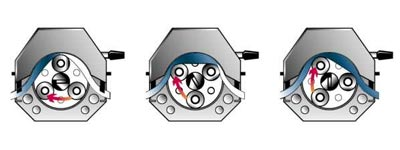
\includegraphics[height=3.5cm]{chap/figure/2-1.jpg}
  \caption{蠕动泵工作原理图}
  \label{fig:2-1}
\end{figure}

蠕动泵的特点明显:一方面,由于运送的材料只接触软管,不接触外界环境,故材料不易受外界环境的污染;其结构决定了蠕动泵的稳定精度好、重复精度高;运送真空度非常高;不需要设置阀门机构,故简化了结构同时又不会出现泄漏现象\supercite{bib4};泵的流道是直通的 没有叶片 阀门等设置因此可用来泵送 易阻塞、含不规则固体颗粒及纤维质物料的流体\supercite{bib4},对运送材料形态要求低;可以输送各种具有磨蚀、腐蚀性,易氧化材料等,运送材料种类广泛。只有软管是需要更换的部件,故更换、维护方便。另一方面,由于蠕动泵使用的软管硬度一定,故其承受压力会受到限制;并且,泵在滚轮交替运作时会产生一个脉冲流,从而导致发生回吸现象,有一定的加样误差。

(2)推入式自动加样结构。推入式自动加样器是以手动加样为原理进行设计的。其动作过程为:从装有样液的试管内吸取一定的试液,移动至加样入口,将试液注入。这种自动加样器设计非常简单,通常只需一根针(上下)移动,样品盘旋转,直到所需的样品瓶位于针下方。使用时,高精度的步进电机带动丝杠配合具导向功能的注射滑块上的传动螺母为动力的传输方式,驱动注射器活塞做往返直线滑动,实现自动精密的定量加样。步进电机在数字脉冲信号响应下,作用于直线轴承实现直线往复运动\supercite{bib5}。此外,注射器的吸入和排出都在步进电机的控制下完成并且采用精密的结构件和合理的驱动方式,此方式可以实现高精度和高准确度,具有良好的稳定性与自动化控制,其结构原理图如\ref{fig:2-2}。

\begin{figure}[htbp!]
  \centering
  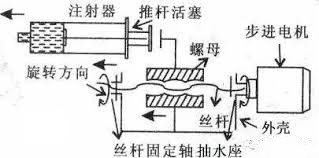
\includegraphics[height=4.8cm]{chap/figure/2-2.jpg}
  \caption{推入式自动加样结构工作原理图}
  \label{fig:2-2}
\end{figure}

(3)六通阀自动加样结构。该结构一般包括两个组成部分:密封垫及固定底座。其大体分为两类:一类是电机驱动的,另一类是用压缩气体驱动的。对于压缩气体驱动结构,利用气动阀内外的压力差,气动阀的一端连接气泵,取样时气动阀内为负压,释放样液时气动阀内为正压。由于采用气动阀,系统要保证良好的气密性,而一旦发生气体泄漏,会对实验分析造成很大的影响,另外气动阀的运动力比电动的会大一些,导致设备噪音大;对于电动结构来说:上部为驱动部分,主要通过程序的执行与否驱动上部。从运动传动角度来看,电动通常属于直接式驱动,气动则属于间接式驱动。

六通阀自动加样结构的加样方法有:部分装液法和完全装液法。采用部分装液法加样时,加样量一般是定量环体积的四分之三,且要保证每次相同的加样体积;采用完全装液法加样时,加样量最少为定量环体积的3至5倍从而保证完全置换样品定量环内残留的溶液以达到所要求的精密度及重现性。为防止缓冲盐和其它残留物质留在加样系统中,每次结束后应冲洗加样器,通常用不含盐的稀释剂、水或不含盐的流动液反复冲洗,再用无纤维纸擦净注射器针头的外侧。由此可知,六通阀自动加样结构对操作人员的加样操作要求高,难以保证加样精度和样液不受外界污染。该结构该结构的工作原理图如\ref{fig:2-3}。

\begin{figure}[htbp!]
  \centering
  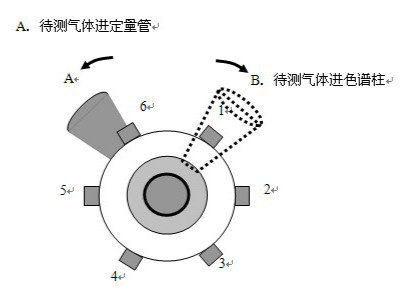
\includegraphics[height=6.5cm]{chap/figure/2-3.jpg}
  \caption{六通阀自动加样结构工作原理图}
  \label{fig:2-3}
\end{figure}

综合比较以上三种加样结构,推入式自动加样结构具有复杂的设计要求,该结构采用丝杠传动且在加样的需求使得步进电机转动方向更换频繁,在此过程中即会出现回程误差,进而造成取样体积出现误差;注射器直接与待检试剂进行接触,不可避免会造成试剂的交叉污染从而造成重大实验损失;此外,该结构零部件更换不方便、难以进行调整以及维护。六通阀自动加样结构的加样阀易于遭受试剂样本中微粒的堵塞和磨损,生命周期短;每次使用前后都要对加样器进行反复的冲洗以避免交叉污染,操作复杂,工作效率低下。此外,六通阀自动加样结构对气密性具有较高的要求,容易受到操作环境变化的影响。而蠕动泵结构操作简单,去离子水和吸入的空气可以有效防止试剂的交叉污染,无加样阀不需要进行密的安全保障;关于运输压力的局限性,我们可以通过增加滚轮的数量降低流量从而降低对软管的压力,使用脉冲抑制器来减少甚至避免液体回吸,脉冲抑制器是一个简单的定位容器,它基于气体可压缩性强于液体可压缩性的工作原理,即脉冲流进入容器、液体上的气袋下陷吸收脉冲进而平缓的流出。当然它的最大缺点是软管易于磨损,但相比于其具有良好的性价比,这是可以接受的。综上所述,本设计的加样结构选用蠕动泵加样结构。

%蠕动泵在工作过程中滚轮会交替挤压软管,当滚轮离开软管%的瞬间会产生回吸现象。当进行加样时回吸现象会严重影响%加样精度,不适用于制造加样精度级高的全自动生化分析仪%。%



















   	% 各章节。
	\chapter{自动加样系统机械臂的设计}
%自动加样系统的一个基本并且关键功用就是在空间内实现任%意位置的准确定位。因此,自动加样系统的加样机械臂的设%计十分重要和关键。本部分完成对其系统结构的设计。
\section{加样机械臂结构类型的选定}
机械臂结构类型多种多样,不同工作场景所使用的机械臂结构形式千差万别。工业上广泛使用的机械臂结构主要有以下几种:

1.铰接式结构:该设计由多个旋转接头和工作臂组成,从简单的双链接结构到多(5-8个以上)相互作用的铰接系统。一般地,该结构在笛卡尔坐标系下能够实现三个转动自由度。一般情况下,铰接结构越多,工作范围越大,机械臂运动也就越精确。铰接式机械臂通常用于装配,压铸,气焊,及喷涂等工作场景。

2.笛卡尔式结构:该结构在笛卡尔坐标系下一般有三个平动自由度,它能实现机械臂在空间内沿着X,Y,Z方向平动从而到达坐标系中任意位置。笛卡尔式机械臂通常用于装载(卸载)工件,印刷电子电路板,材料表面处理等工作场景。该结构提供的工作空间大(可用于其它用途)、控制系统简单。

3.圆柱式结构:该结构在笛卡尔坐标系统能实现沿着X,Y方向平动和绕Z方向转动,机器臂可以移动到由圆柱体描述的体积内的任意位置。该结构在垂直方向上节省了空间,具有良好的刚性能承受较大的有效载荷,但由于其结构限制不能实现360度转动。

4.极坐标式结构:该结构在笛卡尔坐标系下一般能够实现两个旋转自由度和一个平动自由度。相比于圆柱式结构,它在空间内能实现360度的转动,并且在水平方向上的工作距离更长。

根据加样系统的功用和动作流程,加样机械臂要能够到达三维空间中的任意位置;加样多孔板需要放置在工作台上,要求工作台空间足够大;加样液在移送过程中不能有滴漏,要求加样机械臂运动平稳;取样、释样过程不能发生样品(试剂)出错现象,要求加样机械臂运动精度高。考虑以上要素,综合对比上述四种机械臂结构本文选用笛卡尔式结构,该结构能够提供较大的工作空间,控制易于实现,运动平稳且精度高。
\section{驱动方式的选定}
对于机械臂的驱动方式,本文首先考虑使用最为广泛的三种驱动方式:液压驱动、气压驱动、电力驱动,以保证加样机械臂运动的平稳性和位置精确度.

加样机械臂的运动状态是由其驱动系统决定的,它一般由两个部分组成:驱动机构和传动机构。驱动机构其实质可以视为一种能量转换装置,它能将液压能、气动能量、电能等转化为加样机械臂的动能,并通过传动机构使得机械臂动作。根据驱动原理的不同,可以将其分为电力驱动、液压驱动和气压驱动三种类型。

电力驱动:该方式利用电动机产生的力矩和力驱动机械臂进行动作,其具有速度调节范围广、控制精度高、运动平稳性高的特点,具有良好的的控制性和环境适应性。常用的电机驱动器包括直流伺服电机、交流伺服电机、步进电机等。

液压驱动:该方式利用液体产生的压力驱动机械臂进行动作,其具有动力大,无级调速,能实现高速的精度控制等特点。但供油回油等附加元件使其系统体积大,成本高,维修困难,易发生液压油的泄漏而污染环境、稳定性差。该驱动方式多用于矿山机械,重型设备等。

气压驱动:该方式利用气体产生的压力驱动机械臂进行动作,其具有响应快清洁无害,易维护等特点。但其运动稳定性差,功率小,噪声大、难以实现较高精度的位置和速度控制,多用于小功率驱动、运动精度要求低的场合。

自动加样系统实现定量甚至是微量加样,要求其运动平稳性好,位置精度高,运动重复精度好;其部件模块不大、负载小;并且,自动加样系统一般多用于医院、科研机构等对噪声要求严苛的地方。比较上述三种驱动方式,本文选用电力驱动。
\section{传动方式选定}
加样机械臂传动方式对加样精度、稳定性和相应的快速性都产生重要影响。机械系统中传动机构多种多样,本文初步选定将步进电机的回转运动转换成直线运动的滚珠丝杠螺母传动和同步带(工作原理,优点减轻驱动系统重量,简化了其结构)。

滚珠丝杠螺母传动机构与普通丝杠螺母副相似,但其在丝杠和螺母之间装有滚珠。丝杠转动的同时带动滚珠在螺纹滚道里转动,转动的滚珠又将运动传递给螺母使其平动。滚珠丝杠螺母传动机构的传递的效率高,摩擦损失小,传动精度高但是其结构复杂、难以加工、制造成本高;并且滚珠丝杠螺母机构需要润滑和密封机构以提高其工作效率和寿命。

同步带传动是带传动和齿轮传动的有机结合体,兼备二者的优点。同步带的内周表面制有等距的距齿。工作时,利用带与带轮齿之间的啮合关系传递运动\supercite{bib7}。同步带的传动比准确且恒定,带的缓冲吸振特性使其传动平稳,结构紧凑,不需要密封和润滑维护方便,并且重量小,传动能量利用效率高,刚度影响因素少。

加样机械臂的传动比要求较高,传动过程不能发生干涉现象,尽量降低回程误差以提高传动精度,故选取同步带作为传动机构。













































	% 各章节。
	\chapter{自动加样系统硬件系统设计方案的确定}
\section{电机类型的选择}
自动加样系统在加样过程中进行多次重复加样,位置重复性要求好;加样系统必须具有一定的效率,短时间内完成较多的加样任务,速度响应要求要好;加样过程中,为保证测试结果的准确度取样要准,运动平稳性和精度要求高。电力驱动所用的驱动器通常有直流伺服电机、交流伺服电机、步进电机。对于伺服电机,其主要特点是马达或执行机构上装有传感器,传感器将命令执行结果经由伺服放大器传回控制中心,控制中心在比较执行结果和指令值之后再对执行结果进行反馈纠正以不断减小运动执行误差。可以实现转速可以精确控制,速度控制范围广,除了可以进行稳定平顺等速运转之外,还可以根据需求随时变更速度。在极低速度也可以稳定转动。然而,一般伺服电机采取的控制方式是闭环控制,闭环系统中机械结构的惯性、传动误差、变形问题使得控制极其复杂和困难。而步进电机不需要运转量检知器或编码器,且由脉冲信号控制执行机构运动的距离和速度,不需要位置检出和速度检出的回授元件,所以步进电机可正确地依比例跟随脉冲信号而转动,因此就能达成精确的位置和速度控制,且稳定性佳,例外可以通过位置传感器(如限位开关)来辅助位置和速度的控制。综合控制成本和控制效果来看,本文选择步进电机作为$X$、$Y$、$Z$方向平动的驱动器。













	% 各章节。
	\chapter{自动加样系统软件设计方案的确定}

	% 各章节。
	\chapter{自动加样系统机械臂控制的实现}

	%\chapter{自动加样系统软件设计方案的确定}
	% 结论。
	% Copyright (c) 2014,2016 Casper Ti. Vector
% Public domain.

\chapter{论文结论与展望}
\pkuthssffaq % 中文测试文字。

% vim:ts=4:sw=4


	% 正文中的附录部分。
	\appendix
	% 排版参考文献列表。bibintoc 选项使“参考文献”出现在目录中;
	% 如果同时要使参考文献列表参与章节编号,可将“bibintoc”改为“bibnumbered”。
	\printbibliography[heading = bibintoc]
	% 各附录。
	% Copyright (c) 2014,2016 Casper Ti. Vector
% Public domain.

\chapter{附件}
\pkuthssffaq % 中文测试文字。

% vim:ts=4:sw=4


	% 以下为正文之后的部分,默认不进行章节编号。
	\backmatter
	% 致谢。
	% Copyright (c) 2014,2016 Casper Ti. Vector
% Public domain.

\chapter{致谢}
\pkuthssffaq % 中文测试文字。

% vim:ts=4:sw=4

	% 原创性声明和使用授权说明。
	% Copyright (c) 2008-2009 solvethis
% Copyright (c) 2010-2017 Casper Ti. Vector
% All rights reserved.
%
% Redistribution and use in source and binary forms, with or without
% modification, are permitted provided that the following conditions are
% met:
%
% * Redistributions of source code must retain the above copyright notice,
%   this list of conditions and the following disclaimer.
% * Redistributions in binary form must reproduce the above copyright
%   notice, this list of conditions and the following disclaimer in the
%   documentation and/or other materials provided with the distribution.
% * Neither the name of Peking University nor the names of its contributors
%   may be used to endorse or promote products derived from this software
%   without specific prior written permission.
%
% THIS SOFTWARE IS PROVIDED BY THE COPYRIGHT HOLDERS AND CONTRIBUTORS "AS
% IS" AND ANY EXPRESS OR IMPLIED WARRANTIES, INCLUDING, BUT NOT LIMITED TO,
% THE IMPLIED WARRANTIES OF MERCHANTABILITY AND FITNESS FOR A PARTICULAR
% PURPOSE ARE DISCLAIMED. IN NO EVENT SHALL THE COPYRIGHT HOLDER OR
% CONTRIBUTORS BE LIABLE FOR ANY DIRECT, INDIRECT, INCIDENTAL, SPECIAL,
% EXEMPLARY, OR CONSEQUENTIAL DAMAGES (INCLUDING, BUT NOT LIMITED TO,
% PROCUREMENT OF SUBSTITUTE GOODS OR SERVICES; LOSS OF USE, DATA, OR
% PROFITS; OR BUSINESS INTERRUPTION) HOWEVER CAUSED AND ON ANY THEORY OF
% LIABILITY, WHETHER IN CONTRACT, STRICT LIABILITY, OR TORT (INCLUDING
% NEGLIGENCE OR OTHERWISE) ARISING IN ANY WAY OUT OF THE USE OF THIS
% SOFTWARE, EVEN IF ADVISED OF THE POSSIBILITY OF SUCH DAMAGE.

{
	\ctexset{section = {
		format+ = {\centering}, beforeskip = {40bp}, afterskip = {15bp}
	}}

	% 学校书面要求本页面不要页码,但在给出的 Word 模版中又有页码且编入了目录。
	% 此处以 Word 模版为实际标准进行设定。
	\specialchap{中北大学学位论文原创性声明和使用授权说明}
	\mbox{}\vspace*{-3em}
	\section*{原创性声明}

	本人郑重声明:
	所呈交的学位论文,是本人在导师的指导下,独立进行研究工作所取得的成果。
	除文中已经注明引用的内容外,
	本论文不含任何其他个人或集体已经发表或撰写过的作品或成果。
	对本文的研究做出重要贡献的个人和集体,均已在文中以明确方式标明。
	本声明的法律结果由本人承担。
	\vskip 1em
	\rightline{%
		论文作者签名:\hspace{5em}%
		日期:\hspace{2em}年\hspace{2em}月\hspace{2em}日%
	}

	\section*{%
		学位论文使用授权说明\\[-0.33em]
		\textmd{\zihao{5}(必须装订在提交学校图书馆的印刷本)}%
	}

	本人完全了解中北大学关于收集、保存、使用学位论文的规定,即:
	\begin{itemize}
		\item 按照学校要求提交学位论文的印刷本和电子版本;
		\item 学校有权保存学位论文的印刷本和电子版,
			并提供目录检索与阅览服务,在校园网上提供服务;
		\item 学校可以采用影印、缩印、数字化或其它复制手段保存论文;
		\item 因某种特殊原因需要延迟发布学位论文电子版,
			授权学校在 $\Box$\nobreakspace{}一年 /
			$\Box$\nobreakspace{}两年 /
			$\Box$\nobreakspace{}三年以后在校园网上全文发布。
	\end{itemize}
	\centerline{(保密论文在解密后遵守此规定)}
	\vskip 1em
	\rightline{%
		论文作者签名:\hspace{5em}导师签名:\hspace{5em}%
		日期:\hspace{2em}年\hspace{2em}月\hspace{2em}日%
	}

	% 若需排版二维码,请将二维码图片重命名为“barcode”,
	% 转为合适的图片格式,并放在当前目录下,然后去掉下面 2 行的注释。
	%\vfill\noindent
	%\includegraphics[height = 5em]{barcode}
}

% vim:ts=4:sw=4

\end{document}

% vim:ts=4:sw=4
